
\section{Assignment 1: \newline \textit{Latency of CoOps}}
\begin{frame}[fragile]{Assignment 1}
    Measure the latency of the following MPI operations:
    \begin{itemize}
        \item Point to Point communication
        \item Broadcast
        \item Scatter
    \end{itemize}
    We use the OSU Micro-Benchmarks suite.
\end{frame}


%
%   Latency
%
\begin{frame}[fragile,t]{Latency}
    We use the \texttt{osu\_latency} benchmark to measure the latency
    of the Point-to-Point communication between two processes. \\
    We perform this test on three different topologies:
    \begin{itemize}
        \item \textbf{Intra-socket}: same socket, different cores
        \item \textbf{Intra-node}: same node, different sockets
        \item \textbf{Intra-cluster}: different nodes
    \end{itemize}
    We spawn two processes. The first is always bound to core 0.
\end{frame}
\begin{frame}[fragile]{Latency - Intra-socket}
    \begin{multicols}{2}
        \begin{figure}[H]
            \centering
            \resizebox{0.38\textwidth}{!}{
            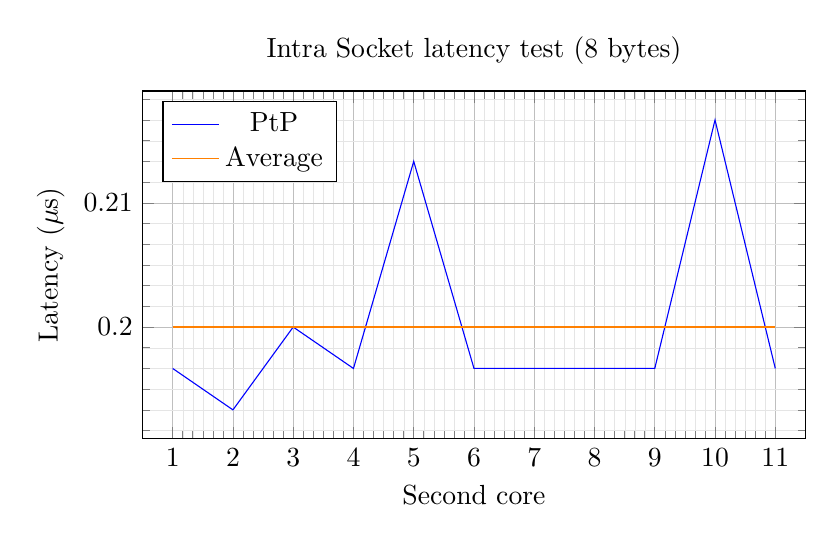
\begin{tikzpicture}
                \begin{axis}[
                    title={Intra Socket latency test (8 bytes)},
                    xlabel={Second core},
                    ylabel={Latency ($\mu$s)},
                    legend pos=north west,
                    grid=both,
                    grid style={line width=.1pt, draw=gray!20},
                    major grid style={line width=.2pt,draw=gray!50},
                    minor tick num=5,
                    xtick={1, 2, 3, 4, 5, 6, 7, 8, 9, 10, 11},
                    % xmode=log,
                    % log basis x={2},
                    % ymin=0,
                    xmin=0.5,
                    xmax=11.5,
                    % xmax=100,
                    % ytick={0, 50, 100, 150, 200, 250, 300, 350, 400},
                    width=10cm,
                    height=6cm,
                    % cycle list name=color list,
                ]
                
                % x = [0,1,...,11]
                % y = [1.23599500e+04 1.96666667e-01 1.93333333e-01 2.00000000e-01 1.96666667e-01 2.13333333e-01 1.96666667e-01 1.96666667e-01 1.96666667e-01 1.96666667e-01 2.16666667e-01 1.96666667e-01]
                % avg = 0.19999999999999998
                % Blue line: Real
                \addplot[
                    color=blue,
                    mark=none,
                    ]
                    coordinates {
                    (1, 0.196667)
                    (2, 0.193333)
                    (3, 0.200000)
                    (4, 0.196667)
                    (5, 0.213333)
                    (6, 0.196667)
                    (7, 0.196667)
                    (8, 0.196667)
                    (9, 0.196667)
                    (10, 0.216667)
                    (11, 0.196667)
                    };
                    \addlegendentry{PtP}
                
                % Orange line: Average
                \addplot[
                    color=orange,
                    mark=none,
                    ]
                    coordinates {
                    (1, 0.19999999999999998)
                    (11, 0.19999999999999998)
                    };
                    \addlegendentry{Average}
                
                \end{axis}
            \end{tikzpicture}
            }
            \resizebox{0.38\textwidth}{!}{
            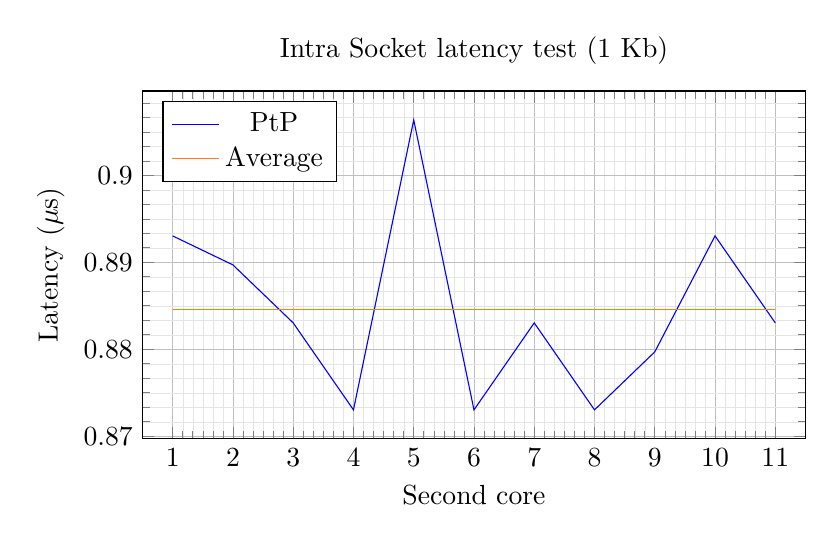
\begin{tikzpicture}
                \begin{axis}[
                    title={Intra Socket latency test (1 Kb)},
                    xlabel={Second core},
                    ylabel={Latency ($\mu$s)},
                    legend pos=north west,
                    grid=both,
                    grid style={line width=.1pt, draw=gray!20},
                    major grid style={line width=.2pt,draw=gray!50},
                    minor tick num=5,
                    xtick={1, 2, 3, 4, 5, 6, 7, 8, 9, 10, 11},
                    % xmode=log,
                    % log basis x={2},
                    % ymin=0,
                    xmin=0.5,
                    xmax=11.5,
                    % xmax=100,
                    % ytick={0, 50, 100, 150, 200, 250, 300, 350, 400},
                    width=10cm,
                    height=6cm,
                    % cycle list name=color list,
                ]
                
                % x = [0,1,...,11]
                % y = [1.25343200e+04 8.93030303e-01 8.89696970e-01 8.83030303e-01 8.73030303e-01 9.06363636e-01 8.73030303e-01 8.83030303e-01 8.73030303e-01 8.79696970e-01 8.93030303e-01 8.83030303e-01 ]
                % avg = 0.8845454545454546
                % Blue line: Real
                \addplot[
                    color=blue,
                    mark=none,
                    ]
                    coordinates {
                    (1, 0.893030)
                    (2, 0.889697)
                    (3, 0.883030)
                    (4, 0.873030)
                    (5, 0.906364)
                    (6, 0.873030)
                    (7, 0.883030)
                    (8, 0.873030)
                    (9, 0.879697)
                    (10, 0.893030)
                    (11, 0.883030)
                    };
                    \addlegendentry{PtP}
                
                % Orange line: Average
                \addplot[
                    color=orange,
                    mark=none,
                    ]
                    coordinates {
                    (1, 0.8845454545454546)
                    (11, 0.8845454545454546)
                    };
                    \addlegendentry{Average}
                
                \end{axis}
            \end{tikzpicture}
            }
            \resizebox{0.38\textwidth}{!}{
            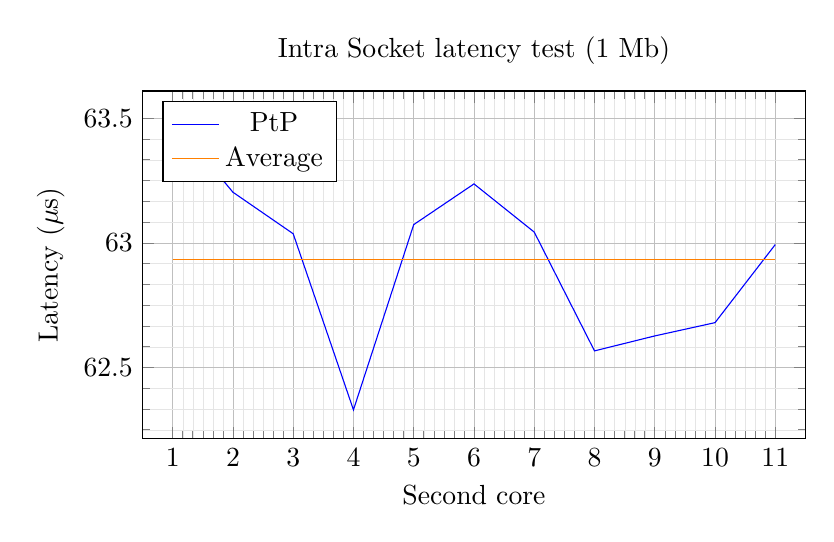
\begin{tikzpicture}
                \begin{axis}[
                    title={Intra Socket latency test (1 Mb)},
                    xlabel={Second core},
                    ylabel={Latency ($\mu$s)},
                    legend pos=north west,
                    grid=both,
                    grid style={line width=.1pt, draw=gray!20},
                    major grid style={line width=.2pt,draw=gray!50},
                    minor tick num=5,
                    xtick={1, 2, 3, 4, 5, 6, 7, 8, 9, 10, 11},
                    % xmode=log,
                    % log basis x={2},
                    % ymin=0,
                    xmin=0.5,
                    xmax=11.5,
                    % xmax=100,
                    % ytick={0, 50, 100, 150, 200, 250, 300, 350, 400},
                    width=10cm,
                    height=6cm,
                    % cycle list name=color list,
                ]
                
                % x = [0,1,...,11]
                % y = [12189.89 63.4930303 63.2030303 63.03636364 62.32969697 63.0730303 63.23636364 63.0430303 62.56636364 62.62636364 62.67969697 62.9930303 ]
                % avg = 62.93454545454545
                % Blue line: Real
                \addplot[
                    color=blue,
                    mark=none,
                    ]
                    coordinates {
                    (1, 63.4930303)
                    (2, 63.2030303)
                    (3, 63.03636364)
                    (4, 62.32969697)
                    (5, 63.0730303)
                    (6, 63.23636364)
                    (7, 63.0430303)
                    (8, 62.56636364)
                    (9, 62.62636364)
                    (10, 62.67969697)
                    (11, 62.9930303)
                    };
                    \addlegendentry{PtP}
                
                % Orange line: Average
                \addplot[
                    color=orange,
                    mark=none,
                    ]
                    coordinates {
                    (1, 62.93454545454545)
                    (11, 62.93454545454545)
                    };
                    \addlegendentry{Average}
                
                \end{axis}
            \end{tikzpicture}
            }
        \end{figure}

        \columnbreak

        \begin{table}[H]
            \centering
            \resizebox{0.45\textwidth}{!}{
            \begin{tabular}{|c|c|c|c|}
                \hline
                \textbf{Message size} & \textbf{Average ($\mu$s)} & \textbf{Std ($\mu$s)} & \textbf{Std/Average} \\
                \hline
                8 bytes & 0.19 & 0.007 & 0.0362 \\
                1 Kb & 0.88 & 0.009 & 0.0111 \\
                1 Mb & 62.93 & 0.33 & 0.005 \\
                \hline
            \end{tabular}
            }
        \end{table}
        The latency become more stable as the message size increases.
        \begin{figure}[H]
            \centering
            \resizebox{0.45\textwidth}{!}{
            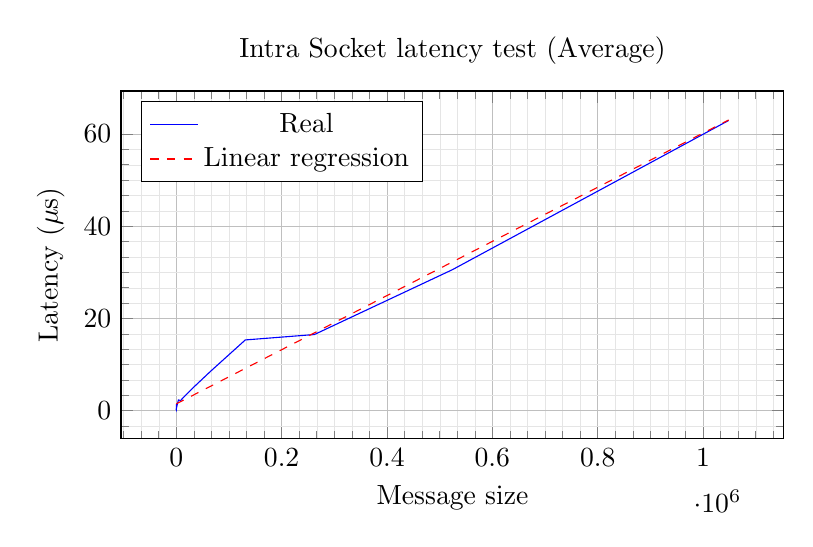
\begin{tikzpicture}
                \begin{axis}[
                    title={Intra Socket latency test (Average)},
                    xlabel={Message size},
                    ylabel={Latency ($\mu$s)},
                    legend pos=north west,
                    grid=both,
                    grid style={line width=.1pt, draw=gray!20},
                    major grid style={line width=.2pt,draw=gray!50},
                    minor tick num=5,
                    % xtick={1, 2, 3, 4, 5, 6, 7, 8, 9, 10, 11},
                    % xmode=log,
                    % log basis x={2},
                    % ymin=0,
                    % xmin=0.5,
                    % xmax=11.5,
                    % xmax=100,
                    % ytick={0, 50, 100, 150, 200, 250, 300, 350, 400},
                    width=10cm,
                    height=6cm,
                    % cycle list name=color list,
                ]
                
                % x = [[      2,       4,       8,      16,      32,      64,     128,     256,           512,    1024,    2048,    4096,    8192,   16384,   32768,   65536, 131072,  262144,  524288, 1048576]
                % y = [ 0.19181818  0.19636364  0.2         0.19090909  0.24090909  0.23272727  1.42545455  0.44272727  0.61818182  0.88454545  1.43636364  2.34272727  2.21636364  3.22181818  5.07454545  8.59727273 15.35272727 16.52272727 30.58909091 62.93454545]
                % linreg = [ 1.49000803  1.49012544  1.49036026  1.49082991  1.49176919  1.49364777  1.49740491  1.5049192   1.51994778  1.55000494  1.61011926  1.73034789  1.97080516  2.45171971  3.4135488   5.33720697  9.18452332 16.87915602 32.26842142 63.04695221]
                % Blue line: Real
                \addplot[
                    color=blue,
                    mark=none,
                    ]
                    coordinates {
                    (2, 0.19181818)
                    (4, 0.19636364)
                    (8, 0.2)
                    (16, 0.19090909)
                    (32, 0.24090909)
                    (64, 0.23272727)
                    (128, 1.42545455)
                    (256, 0.44272727)
                    (512, 0.61818182)
                    (1024, 0.88454545)
                    (2048, 1.43636364)
                    (4096, 2.34272727)
                    (8192, 2.21636364)
                    (16384, 3.22181818)
                    (32768, 5.07454545)
                    (65536, 8.59727273)
                    (131072, 15.35272727)
                    (262144, 16.52272727)
                    (524288, 30.58909091)
                    (1048576, 62.93454545)
                    };
                \addlegendentry{Real}
    
                % Red line: Linear regression
                % dashe
                \addplot[
                    color=red,
                    mark=none,
                    dashed
                    ]
                    coordinates {
                    (2, 1.49000803)
                    (4, 1.49012544)
                    (8, 1.49036026)
                    (16, 1.49082991)
                    (32, 1.49176919)
                    (64, 1.49364777)
                    (128, 1.49740491)
                    (256, 1.5049192)
                    (512, 1.51994778)
                    (1024, 1.55000494)
                    (2048, 1.61011926)
                    (4096, 1.73034789)
                    (8192, 1.97080516)
                    (16384, 2.45171971)
                    (32768, 3.4135488)
                    (65536, 5.33720697)
                    (131072, 9.18452332)
                    (262144, 16.87915602)
                    (524288, 32.26842142)
                    (1048576, 63.04695221)
                    };
                \addlegendentry{Linear regression}
                
                \end{axis}
            \end{tikzpicture}
            }
            $\beta_1$: $58.7 \mu$s/MB, $\beta_0$: $1.49 \mu$s.
        \end{figure}
    \end{multicols}
\end{frame}
\begin{frame}[fragile]{Latency - Intra-node}
    \begin{multicols}{2}
        \begin{figure}[H]
            \centering
            \resizebox{0.45\textwidth}{!}{
            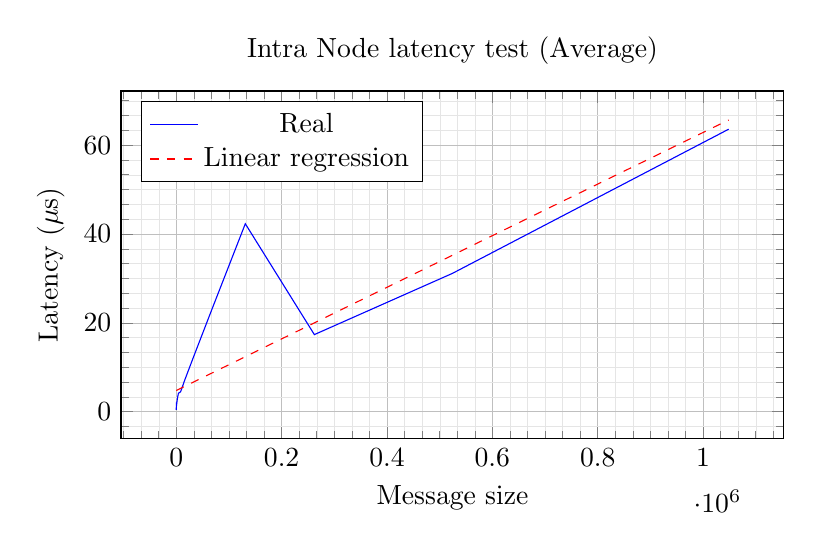
\begin{tikzpicture}
                \begin{axis}[
                    title={Intra Node latency test (Average)},
                    xlabel={Message size},
                    ylabel={Latency ($\mu$s)},
                    legend pos=north west,
                    grid=both,
                    grid style={line width=.1pt, draw=gray!20},
                    major grid style={line width=.2pt,draw=gray!50},
                    minor tick num=5,
                    % xtick={1, 2, 3, 4, 5, 6, 7, 8, 9, 10, 11},
                    % xmode=log,
                    % log basis x={2},
                    % ymin=0,
                    % xmin=0.5,
                    % xmax=11.5,
                    % xmax=100,
                    % ytick={0, 50, 100, 150, 200, 250, 300, 350, 400},
                    width=10cm,
                    height=6cm,
                    % cycle list name=color list,
                ]
                
                % x = [[      2,       4,       8,      16,      32,      64,     128,     256,           512,    1024,    2048,    4096,    8192,   16384,   32768,   65536, 131072,  262144,  524288, 1048576]
                % y = [ 0.41        0.4         0.40666667  0.41333333  0.57        0.58  2.08333333  1.14666667  1.42666667  1.92666667  2.85333333  4.14666667  4.46        7.20333333 12.32       22.38666667 42.30333333 17.35 31.13333333 63.58666667]
                % linreg = [ 4.76505022  4.76516638  4.76539871  4.76586337  4.76679269  4.76865134  4.77236863  4.7798032   4.79467236  4.82441066  4.88388727  5.0028405  5.24074695  5.71655985  6.66818564  8.57143723 12.37794041 19.99094678 35.21695951 65.66898497]
                % Blue line: Real
                \addplot[
                    color=blue,
                    mark=none,
                    ]
                    coordinates {
                    (2, 0.41)
                    (4, 0.4)
                    (8, 0.40666667)
                    (16, 0.41333333)
                    (32, 0.57)
                    (64, 0.58)
                    (128, 2.08333333)
                    (256, 1.14666667)
                    (512, 1.42666667)
                    (1024, 1.92666667)
                    (2048, 2.85333333)
                    (4096, 4.14666667)
                    (8192, 4.46)
                    (16384, 7.20333333)
                    (32768, 12.32)
                    (65536, 22.38666667)
                    (131072, 42.30333333)
                    (262144, 17.35)
                    (524288, 31.13333333)
                    (1048576, 63.58666667)
                    };
                \addlegendentry{Real}
    
                % Red line: Linear regression
                % dashe
                \addplot[
                    color=red,
                    mark=none,
                    dashed
                    ]
                    coordinates {
                    (2, 4.76505022)
                    (4, 4.76516638)
                    (8, 4.76539871)
                    (16, 4.76586337)
                    (32, 4.76679269)
                    (64, 4.76865134)
                    (128, 4.77236863)
                    (256, 4.7798032)
                    (512, 4.79467236)
                    (1024, 4.82441066)
                    (2048, 4.88388727)
                    (4096, 5.0028405)
                    (8192, 5.24074695)
                    (16384, 5.71655985)
                    (32768, 6.66818564)
                    (65536, 8.57143723)
                    (131072, 12.37794041)
                    (262144, 19.99094678)
                    (524288, 35.21695951)
                    (1048576, 65.66898497)
                    };
                \addlegendentry{Linear regression}
                
                \end{axis}
            \end{tikzpicture}
            }
            $\beta_1$: $58.7 \mu$s/MB, $\beta_0$: $4.76 \mu$s.
        \end{figure}
        \begin{table}[H]
            \centering
            \resizebox{0.45\textwidth}{!}{
            \begin{tabular}{|c|c|c|c|}
                \hline
                \textbf{Message size} & \textbf{Average ($\mu$s)} & \textbf{Std ($\mu$s)} & \textbf{Std/Average} \\
                \hline
                8 bytes & 0.405 & 0.005 & 0.0123 \\
                1 Kb & 1.9175 & 0.0217 & 0.0113 \\
                1 Mb & 63.6575 & 0.8918 & 0.0140 \\
                \hline
            \end{tabular}
            }
        \end{table}

        \columnbreak

        The slope is the same as the intra-socket test, but the intercept is
        higher. \\
        Higher overhead at low message sizes.
    \end{multicols}
\end{frame}
\begin{frame}[fragile]{Latency - Intra-cluster}
    \begin{multicols}{2}
        \begin{figure}[H]
            \centering
            \resizebox{0.45\textwidth}{!}{
            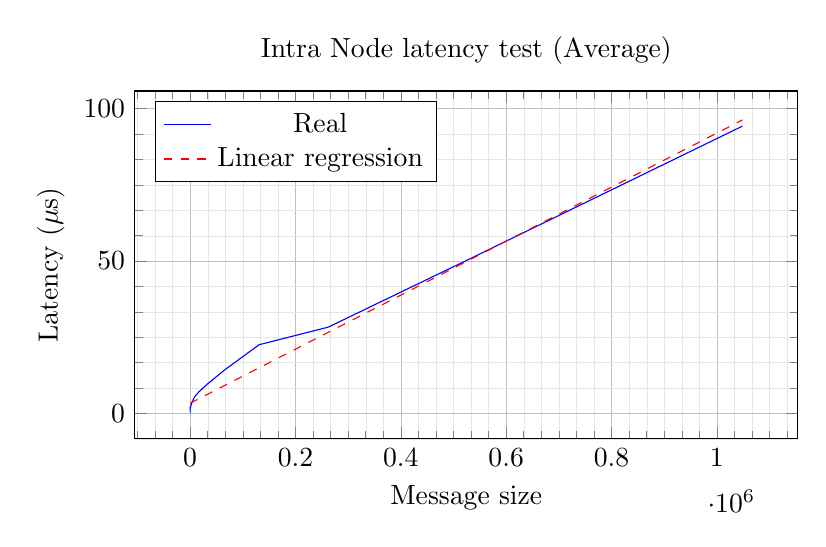
\begin{tikzpicture}
                \begin{axis}[
                    title={Intra Node latency test (Average)},
                    xlabel={Message size},
                    ylabel={Latency ($\mu$s)},
                    legend pos=north west,
                    grid=both,
                    grid style={line width=.1pt, draw=gray!20},
                    major grid style={line width=.2pt,draw=gray!50},
                    minor tick num=5,
                    % xtick={1, 2, 3, 4, 5, 6, 7, 8, 9, 10, 11},
                    % xmode=log,
                    % log basis x={2},
                    % ymin=0,
                    % xmin=0.5,
                    % xmax=11.5,
                    % xmax=100,
                    % ytick={0, 50, 100, 150, 200, 250, 300, 350, 400},
                    width=10cm,
                    height=6cm,
                    % cycle list name=color list,
                ]
                
                % x = [[      2,       4,       8,      16,      32,      64,     128,     256,           512,    1024,    2048,    4096,    8192,   16384,   32768,   65536, 131072,  262144,  524288, 1048576]
                % y = [ 1.16666667  1.13333333  1.14333333  1.13666667  1.19333333  1.41  1.5         1.74        1.83        2.02333333  2.80666667  3.79666667  5.32666667  7.01333333  9.60333333 14.25       22.52666667 28.29333333 50.15666667 94.30333333]
                % linreg = [ 3.31773287  3.31791025  3.31826502  3.31897457  3.32039365  3.32323182  3.32890816  3.34026085  3.36296622  3.40837696  3.49919845  3.68084142  4.04412736  4.77069924  6.223843    9.13013051 14.94270555 26.56785562 49.81815576 96.31875605]
                % Blue line: Real
                \addplot[
                    color=blue,
                    mark=none,
                    ]
                    coordinates {
                    (2, 1.16666667)
                    (4, 1.13333333)
                    (8, 1.14333333)
                    (16, 1.13666667)
                    (32, 1.19333333)
                    (64, 1.41)
                    (128, 1.5)
                    (256, 1.74)
                    (512, 1.83)
                    (1024, 2.02333333)
                    (2048, 2.80666667)
                    (4096, 3.79666667)
                    (8192, 5.32666667)
                    (16384, 7.01333333)
                    (32768, 9.60333333)
                    (65536, 14.25)
                    (131072, 22.52666667)
                    (262144, 28.29333333)
                    (524288, 50.15666667)
                    (1048576, 94.30333333)
                    };
                \addlegendentry{Real}
    
                % Red line: Linear regression
                % dashe
                \addplot[
                    color=red,
                    mark=none,
                    dashed
                    ]
                    coordinates {
                    (2, 3.31773287)
                    (4, 3.31791025)
                    (8, 3.31826502)
                    (16, 3.31897457)
                    (32, 3.32039365)
                    (64, 3.32323182)
                    (128, 3.32890816)
                    (256, 3.34026085)
                    (512, 3.36296622)
                    (1024, 3.40837696)
                    (2048, 3.49919845)
                    (4096, 3.68084142)
                    (8192, 4.04412736)
                    (16384, 4.77069924)
                    (32768, 6.223843)
                    (65536, 9.13013051)
                    (131072, 14.94270555)
                    (262144, 26.56785562)
                    (524288, 49.81815576)
                    (1048576, 96.31875605)
                    };
                \addlegendentry{Linear regression}
                
                \end{axis}
            \end{tikzpicture}
            }
            $\beta_1$: $88,69 \mu$s/MB, $\beta_0$: $3.16 \mu$s.
        \end{figure}
        \begin{table}[H]
            \centering
            \resizebox{0.45\textwidth}{!}{
            \begin{tabular}{|c|c|c|c|}
                \hline
                \textbf{Message size} & \textbf{Average ($\mu$s)} & \textbf{Std ($\mu$s)} & \textbf{Std/Average} \\
                \hline
                8 bytes & 1.1250 & 0.0622 & 0.0553 \\
                1 Kb & 1.9550 & 0.1484 & 0.0759 \\
                1 Mb & 94.2250 & 0.3829 & 0.0041 \\
                \hline
            \end{tabular}
            }
        \end{table}

        \columnbreak

        Higher slope and intercept. \\
        Less overhead at low message sizes.
    \end{multicols}
\end{frame}

%
%   Broadcast
%
\begin{frame}[fragile]{Broadcast}
    We use the \texttt{osu\_bcast} benchmark to measure the latency
    of the Broadcast operation. Sending data from the root process
    to every other process. \\
    Distribiution algorithms:
    \begin{enumerate}
        \item Basic Linear
        \item Chain
        \item Binary Tree
        \item Binomial Tree
    \end{enumerate}
\end{frame}
\begin{frame}[fragile]{Broadcast algorithms}
    \textbf{Basic Linear}: \\
    The root process sends the data to every other process in 
    a round-robin fashion. \\
    Number of steps: $n-1$.
    \vspace*{.25cm}
    \textbf{Chain}: \\
    The root process sends the data to the next process, which forwards
    the data to the next process, and so on. \\
    Number of steps: $n-1$.
    \vspace*{.25cm}
    \textbf{Binary Tree}: \\
    The data is divided in chunks. The root process sends the first two
    to two different processes. Each of these processes sends the data
    to two other processes, and so on. \\
    Number of steps: $\log_2(n)$.
\end{frame}
\begin{frame}[fragile]{Broadcast algorithms}
    \textbf{Binomial Tree}: \\
    Each process communicates with a subset of other processes.
    \begin{enumerate}
        \item[$t_0:$] $P_0$ $\rightarrow$ $P_1$,
        \item[$t_1:$] $P_0$ $\rightarrow$ $P_1$, $P_2$ $\rightarrow$ $P_3$,
        \item[$t_2:$] $P_0$ $\rightarrow$ $P_4$, $P_2$ $\rightarrow$ $P_5$, $P_3$ $\rightarrow$ $P_6$,
        \item[$t_3:$] \dots
    \end{enumerate}
    Number of steps: $\log_2(n)$. Data transmitted: $(n-1) \cdot m$.
\end{frame}
\begin{frame}[fragile]{Broadcast}
    \begin{multicols}{2}
        \begin{figure}[H]
            \centering
            \resizebox{0.38\textwidth}{!}{
            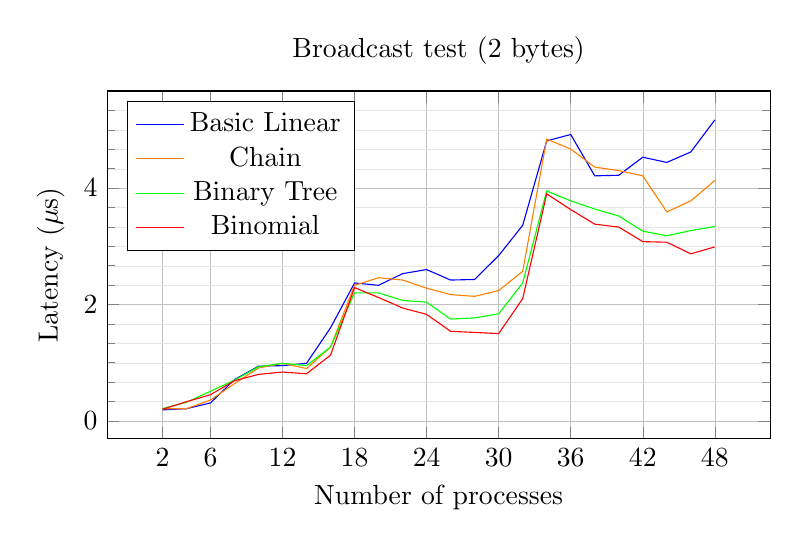
\begin{tikzpicture}
                \begin{axis}[
                    title={Broadcast test (2 bytes)},
                    xlabel={Number of processes},
                    ylabel={Latency ($\mu$s)},
                    legend pos=north west,
                    grid=both,
                    grid style={line width=.1pt, draw=gray!20},
                    major grid style={line width=.2pt,draw=gray!50},
                    minor tick num=5,
                    xtick={2, 6, 12, 18, 24, 30, 36, 42, 48},
                    % xmode=log,
                    % log basis x={2},
                    % ymin=0,
                    % xmin=0.5,
                    % xmax=11.5,
                    % xmax=100,
                    % ytick={0, 50, 100, 150, 200, 250, 300, 350, 400},
                    width=10cm,
                    height=6cm,
                    % cycle list name=color list,
                ]
                
                % x = [ 2  4  6  8 10 12 14 16 18 20 22 24 26 28 30 32 34 36 38 40 42 44 46 48]
                % basic-linear = [0.19 0.21 0.31 0.71 0.94 0.95 0.99 1.6  2.37 2.33 2.53 2.6  2.42 2.43 2.84 3.36 4.81 4.92 4.21 4.22 4.53 4.44 4.62 5.17]
                % chain = [0.21 0.21 0.36 0.64 0.91 0.99 0.9  1.27 2.33 2.46 2.42 2.28 2.17 2.14  2.24 2.57 4.84 4.67 4.36 4.3  4.21 3.59 3.78 4.13]
                % binary-tree = [0.21 0.32 0.51 0.7  0.93 0.99 0.95 1.27 2.2  2.2  2.07 2.04 1.75 1.77  1.84 2.37 3.95 3.78 3.64 3.52 3.26 3.18 3.27 3.34]
                % binomial = [0.2  0.33 0.45 0.69 0.8  0.84 0.81 1.13 2.29 2.12 1.94 1.83 1.54 1.52  1.5  2.1  3.9  3.63 3.38 3.33 3.08 3.07 2.87 2.99]
                
                % Blue line: basic-linear
                \addplot[
                    color=blue,
                    mark=none,
                    ]
                    coordinates {
                    (2, 0.19)
                    (4, 0.21)
                    (6, 0.31)
                    (8, 0.71)
                    (10, 0.94)
                    (12, 0.95)
                    (14, 0.99)
                    (16, 1.6)
                    (18, 2.37)
                    (20, 2.33)
                    (22, 2.53)
                    (24, 2.6)
                    (26, 2.42)
                    (28, 2.43)
                    (30, 2.84)
                    (32, 3.36)
                    (34, 4.81)
                    (36, 4.92)
                    (38, 4.21)
                    (40, 4.22)
                    (42, 4.53)
                    (44, 4.44)
                    (46, 4.62)
                    (48, 5.17)
                    };
                    \addlegendentry{Basic Linear}
    
                % Orange line: chain
                \addplot[
                    color=orange,
                    mark=none,
                    ]
                    coordinates {
                    (2, 0.21)
                    (4, 0.21)
                    (6, 0.36)
                    (8, 0.64)
                    (10, 0.91)
                    (12, 0.99)
                    (14, 0.9)
                    (16, 1.27)
                    (18, 2.33)
                    (20, 2.46)
                    (22, 2.42)
                    (24, 2.28)
                    (26, 2.17)
                    (28, 2.14)
                    (30, 2.24)
                    (32, 2.57)
                    (34, 4.84)
                    (36, 4.67)
                    (38, 4.36)
                    (40, 4.3)
                    (42, 4.21)
                    (44, 3.59)
                    (46, 3.78)
                    (48, 4.13)
                    };
                    \addlegendentry{Chain}
    
                % Green line: binary-tree
                \addplot[
                    color=green,
                    mark=none,
                    ]
                    coordinates {
                    (2, 0.21)
                    (4, 0.32)
                    (6, 0.51)
                    (8, 0.7)
                    (10, 0.93)
                    (12, 0.99)
                    (14, 0.95)
                    (16, 1.27)
                    (18, 2.2)
                    (20, 2.2)
                    (22, 2.07)
                    (24, 2.04)
                    (26, 1.75)
                    (28, 1.77)
                    (30, 1.84)
                    (32, 2.37)
                    (34, 3.95)
                    (36, 3.78)
                    (38, 3.64)
                    (40, 3.52)
                    (42, 3.26)
                    (44, 3.18)
                    (46, 3.27)
                    (48, 3.34)
                    };
                    \addlegendentry{Binary Tree}
    
                % Red line: binomial
                \addplot[
                    color=red,
                    mark=none,
                    ]
                    coordinates {
                    (2, 0.2)
                    (4, 0.33)
                    (6, 0.45)
                    (8, 0.69)
                    (10, 0.8)
                    (12, 0.84)
                    (14, 0.81)
                    (16, 1.13)
                    (18, 2.29)
                    (20, 2.12)
                    (22, 1.94)
                    (24, 1.83)
                    (26, 1.54)
                    (28, 1.52)
                    (30, 1.5)
                    (32, 2.1)
                    (34, 3.9)
                    (36, 3.63)
                    (38, 3.38)
                    (40, 3.33)
                    (42, 3.08)
                    (44, 3.07)
                    (46, 2.87)
                    (48, 2.99)
                    };
                    \addlegendentry{Binomial}
                
                \end{axis}
            \end{tikzpicture}
            }
            \resizebox{0.38\textwidth}{!}{
            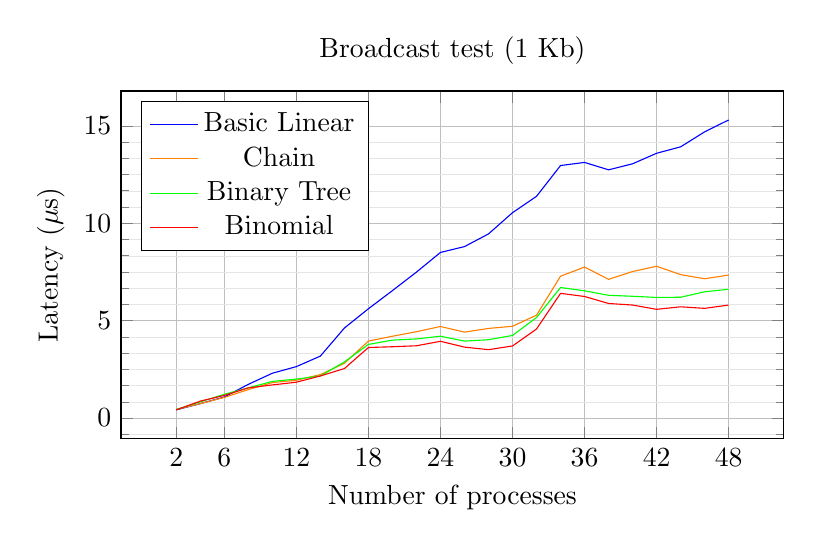
\begin{tikzpicture}
                \begin{axis}[
                    title={Broadcast test (1 Kb)},
                    xlabel={Number of processes},
                    ylabel={Latency ($\mu$s)},
                    legend pos=north west,
                    grid=both,
                    grid style={line width=.1pt, draw=gray!20},
                    major grid style={line width=.2pt,draw=gray!50},
                    minor tick num=5,
                    xtick={2, 6, 12, 18, 24, 30, 36, 42, 48},
                    % xmode=log,
                    % log basis x={2},
                    % ymin=0,
                    % xmin=0.5,
                    % xmax=11.5,
                    % xmax=100,
                    % ytick={0, 50, 100, 150, 200, 250, 300, 350, 400},
                    width=10cm,
                    height=6cm,
                    % cycle list name=color list,
                ]
                
                % x = [ 2  4  6  8 10 12 14 16 18 20 22 24 26 28 30 32 34 36 38 40 42 44 46 48]
                % basic-linear = [ 0.42  0.74  1.08  1.73  2.3   2.64  3.18  4.62  5.61  6.54  7.49  8.5 8.8   9.45 10.54 11.38 12.96 13.12 12.74 13.05 13.59 13.92 14.69 15.3 ]
                % chain = [0.44 0.74 1.06 1.46 1.82 1.94 2.23 2.81 3.95 4.2  4.43 4.7  4.41 4.6 4.71 5.28 7.28 7.75 7.12 7.52 7.79 7.36 7.15 7.34]
                % binary-tree = [0.44 0.83 1.22 1.55 1.88 2.   2.16 2.88 3.78 4.   4.06 4.2  3.95 4.02 4.24 5.16 6.7  6.53 6.3  6.25 6.19 6.2  6.48 6.61]
                % binomial = [0.42 0.87 1.16 1.55 1.7  1.84 2.16 2.54 3.62 3.66 3.71 3.94 3.64 3.51 3.7  4.57 6.4  6.24 5.88 5.8  5.58 5.71 5.63 5.8 ]
                
                % Blue line: basic-linear
                \addplot[
                    color=blue,
                    mark=none,
                    ]
                    coordinates {
                    (2, 0.42)
                    (4, 0.74)
                    (6, 1.08)
                    (8, 1.73)
                    (10, 2.3)
                    (12, 2.64)
                    (14, 3.18)
                    (16, 4.62)
                    (18, 5.61)
                    (20, 6.54)
                    (22, 7.49)
                    (24, 8.5)
                    (26, 8.8)
                    (28, 9.45)
                    (30, 10.54)
                    (32, 11.38)
                    (34, 12.96)
                    (36, 13.12)
                    (38, 12.74)
                    (40, 13.05)
                    (42, 13.59)
                    (44, 13.92)
                    (46, 14.69)
                    (48, 15.3)
                    };
                    \addlegendentry{Basic Linear}
    
                % Orange line: chain
                \addplot[
                    color=orange,
                    mark=none,
                    ]
                    coordinates {
                    (2, 0.44)
                    (4, 0.74)
                    (6, 1.06)
                    (8, 1.46)
                    (10, 1.82)
                    (12, 1.94)
                    (14, 2.23)
                    (16, 2.81)
                    (18, 3.95)
                    (20, 4.2)
                    (22, 4.43)
                    (24, 4.7)
                    (26, 4.41)
                    (28, 4.6)
                    (30, 4.71)
                    (32, 5.28)
                    (34, 7.28)
                    (36, 7.75)
                    (38, 7.12)
                    (40, 7.52)
                    (42, 7.79)
                    (44, 7.36)
                    (46, 7.15)
                    (48, 7.34)
                    };
                    \addlegendentry{Chain}
    
                % Green line: binary-tree
                \addplot[
                    color=green,
                    mark=none,
                    ]
                    coordinates {
                    (2, 0.44)
                    (4, 0.83)
                    (6, 1.22)
                    (8, 1.55)
                    (10, 1.88)
                    (12, 2)
                    (14, 2.16)
                    (16, 2.88)
                    (18, 3.78)
                    (20, 4)
                    (22, 4.06)
                    (24, 4.2)
                    (26, 3.95)
                    (28, 4.02)
                    (30, 4.24)
                    (32, 5.16)
                    (34, 6.7)
                    (36, 6.53)
                    (38, 6.3)
                    (40, 6.25)
                    (42, 6.19)
                    (44, 6.2)
                    (46, 6.48)
                    (48, 6.61)
                    };
                    \addlegendentry{Binary Tree}
    
                % Red line: binomial
                \addplot[
                    color=red,
                    mark=none,
                    ]
                    coordinates {
                    (2, 0.42)
                    (4, 0.87)
                    (6, 1.16)
                    (8, 1.55)
                    (10, 1.7)
                    (12, 1.84)
                    (14, 2.16)
                    (16, 2.54)
                    (18, 3.62)
                    (20, 3.66)
                    (22, 3.71)
                    (24, 3.94)
                    (26, 3.64)
                    (28, 3.51)
                    (30, 3.7)
                    (32, 4.57)
                    (34, 6.4)
                    (36, 6.24)
                    (38, 5.88)
                    (40, 5.8)
                    (42, 5.58)
                    (44, 5.71)
                    (46, 5.63)
                    (48, 5.8)
                    };
                    \addlegendentry{Binomial}
                
                \end{axis}
            \end{tikzpicture}
            }
            % \resizebox{0.38\textwidth}{!}{
            % \begin{tikzpicture}
            %     \begin{axis}[
            %         title={Broadcast test (1 Mb)},
            %         xlabel={Number of processes},
            %         ylabel={Latency ($\mu$s)},
            %         legend pos=north west,
            %         grid=both,
            %         grid style={line width=.1pt, draw=gray!20},
            %         major grid style={line width=.2pt,draw=gray!50},
            %         minor tick num=5,
            %         xtick={2, 6, 12, 18, 24, 30, 36, 42, 48},
            %         % xmode=log,
            %         % log basis x={2},
            %         % ymin=0,
            %         % xmin=0.5,
            %         % xmax=11.5,
            %         % xmax=100,
            %         % ytick={0, 50, 100, 150, 200, 250, 300, 350, 400},
            %         width=10cm,
            %         height=6cm,
            %         % cycle list name=color list,
            %     ]
                
            %     % x = [ 2  4  6  8 10 12 14 16 18 20 22 24 26 28 30 32 34 36 38 40 42 44 46 48]
            %     % basic-linear = [  62.3   184.64  340.23  441.34  485.99  639.43  737.9   997.37 1113.78 1416.71 1553.68 1812.4  1699.96 1634.78 1550.19 1443.08 1433.01 1570.21 1455.46 1640.05 1625.38 1698.98 1789.84 1819.08]
            %     % chain = [  61.81  205.71  319.63  373.89  470.52  465.78  571.05  668.8   798.57  789.29  806.91  915.37  961.03  991.41  963.26  918.78  917.56 1023.86  1000.39 1101.16 1108.08 1100.23 1048.36 1074.3 ]
            %     % binary-tree = [  63.35  193.11  306.55  370.21  436.4   503.01  595.54  683.32  761.52  842.13  840.07  880.99  881.86  865.36  907.51 1033.67 1124.8  1249.66  1431.95 1609.93 1656.84 1668.19 1661.83 1719.17]
            %     % binomial = [  62.29  184.39  345.75  387.37  481.63  536.61  575.96  662.77  909.46 1029.22  990.14 1050.39 1078.56 1044.28 1118.66 1111.21 1062.79 1020.77 1023.83 1148.91 1219.63 1314.8  1462.38 1537.52]
                
            %     % Blue line: basic-linear
            %     \addplot[
            %         color=blue,
            %         mark=none,
            %         ]
            %         coordinates {
            %         (2, 62.3)
            %         (4, 184.64)
            %         (6, 340.23)
            %         (8, 441.34)
            %         (10, 485.99)
            %         (12, 639.43)
            %         (14, 737.9)
            %         (16, 997.37)
            %         (18, 1113.78)
            %         (20, 1416.71)
            %         (22, 1553.68)
            %         (24, 1812.4)
            %         (26, 1699.96)
            %         (28, 1634.78)
            %         (30, 1550.19)
            %         (32, 1443.08)
            %         (34, 1433.01)
            %         (36, 1570.21)
            %         (38, 1455.46)
            %         (40, 1640.05)
            %         (42, 1625.38)
            %         (44, 1698.98)
            %         (46, 1789.84)
            %         (48, 1819.08)
            %         };
            %         \addlegendentry{Basic Linear}
    
            %     % Orange line: chain
            %     \addplot[
            %         color=orange,
            %         mark=none,
            %         ]
            %         coordinates {
            %         (2, 61.81)
            %         (4, 205.71)
            %         (6, 319.63)
            %         (8, 373.89)
            %         (10, 470.52)
            %         (12, 465.78)
            %         (14, 571.05)
            %         (16, 668.8)
            %         (18, 798.57)
            %         (20, 789.29)
            %         (22, 806.91)
            %         (24, 915.37)
            %         (26, 961.03)
            %         (28, 991.41)
            %         (30, 963.26)
            %         (32, 918.78)
            %         (34, 917.56)
            %         (36, 1023.86)
            %         (38, 1000.39)
            %         (40, 1101.16)
            %         (42, 1108.08)
            %         (44, 1100.23)
            %         (46, 1048.36)
            %         (48, 1074.3)
            %         };
            %         \addlegendentry{Chain}
    
            %     % Green line: binary-tree
            %     \addplot[
            %         color=green,
            %         mark=none,
            %         ]
            %         coordinates {
            %         (2, 63.35)
            %         (4, 193.11)
            %         (6, 306.55)
            %         (8, 370.21)
            %         (10, 436.4)
            %         (12, 503.01)
            %         (14, 595.54)
            %         (16, 683.32)
            %         (18, 761.52)
            %         (20, 842.13)
            %         (22, 840.07)
            %         (24, 880.99)
            %         (26, 881.86)
            %         (28, 865.36)
            %         (30, 907.51)
            %         (32, 1033.67)
            %         (34, 1124.8)
            %         (36, 1249.66)
            %         (38, 1431.95)
            %         (40, 1609.93)
            %         (42, 1656.84)
            %         (44, 1668.19)
            %         (46, 1661.83)
            %         (48, 1719.17)
            %         };
            %         \addlegendentry{Binary Tree}
    
            %     % Red line: binomial
            %     \addplot[
            %         color=red,
            %         mark=none,
            %         ]
            %         coordinates {
            %         (2, 62.29)
            %         (4, 184.39)
            %         (6, 345.75)
            %         (8, 387.37)
            %         (10, 481.63)
            %         (12, 536.61)
            %         (14, 575.96)
            %         (16, 662.77)
            %         (18, 909.46)
            %         (20, 1029.22)
            %         (22, 990.14)
            %         (24, 1050.39)
            %         (26, 1078.56)
            %         (28, 1044.28)
            %         (30, 1118.66)
            %         (32, 1111.21)
            %         (34, 1062.79)
            %         (36, 1020.77)
            %         (38, 1023.83)
            %         (40, 1148.91)
            %         (42, 1219.63)
            %         (44, 1314.8)
            %         (46, 1462.38)
            %         (48, 1537.52)
            %         };
            %         \addlegendentry{Binomial}
                
                
            %     \end{axis}
            % \end{tikzpicture}
            % }
        \end{figure}

        \columnbreak

        Especially at low message size, we can notice the two main
        transitions in the latency:
        \begin{itemize}
            \item At 12 processes the first socket is filled
            \item at 24 processes the first node is filled
        \end{itemize}

        After each spike, the latency slightly decreases.
    \end{multicols}
\end{frame}

%
%   Scatter
%
\begin{frame}[fragile]{Scatter}
    We use the \texttt{osu\_scatter} benchmark to measure the latency
    of the Scatter operation. Sending a partition of the data from the
    root process to every other process. \\
    Distribution algorithms:
    \begin{enumerate}
        \item Basic Linear
        \item Binomial Tree
    \end{enumerate}
\end{frame}
\begin{frame}[fragile]{Scatter algorithms}
    \textbf{Basic Linear}: \\
    The root process sends the specific data chunk to each process
    in a round-robin fashion. \\
    Number of steps: $n-1$. \\
    \vspace*{.25cm}
    \textbf{Binomial Tree}: \\
    The root process sends a subset of the data to a subset of processes.
    Assume $P_0$ holds an array divided
    into $8$ chunks $[ c_0, \dots, c_7 ]$ and $P_1, \dots, p_7$ are
    the other processes.
    \begin{enumerate}
        \item[$t_0:$] $P_0$ $\xrightarrow{c_4,\dots,c_7}$ $P_1$,
        \item[$t_1:$] $P_0$ $\xrightarrow{c_2,c_3}$ $P_2$, $P_1$ $\xrightarrow{c_6,c_7}$ $P_3$,
        \item[$t_2:$] $P_0$ $\xrightarrow{c_1}$ $P_4$, $P_1$ $\xrightarrow{c_5}$ $P_6$, $P_2$ $\xrightarrow{c_4}$ $P_5$, $P_3$ $\xrightarrow{c_7}$ $P_7$,
    \end{enumerate}
\end{frame}
\begin{frame}[fragile]{Scatter}
    \begin{multicols}{2}
        \begin{figure}[H]
            \centering
            \resizebox{0.38\textwidth}{!}{
            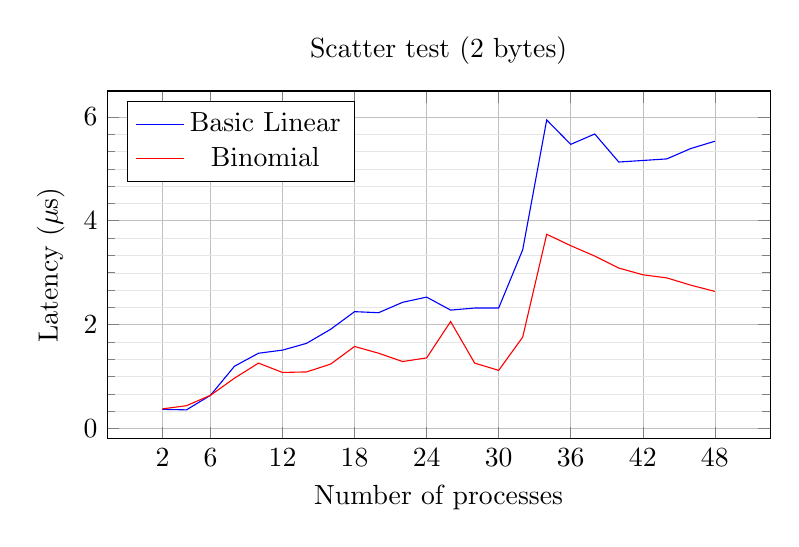
\begin{tikzpicture}
                \begin{axis}[
                    title={Scatter test (2 bytes)},
                    xlabel={Number of processes},
                    ylabel={Latency ($\mu$s)},
                    legend pos=north west,
                    grid=both,
                    grid style={line width=.1pt, draw=gray!20},
                    major grid style={line width=.2pt,draw=gray!50},
                    minor tick num=5,
                    xtick={2, 6, 12, 18, 24, 30, 36, 42, 48},
                    % xmode=log,
                    % log basis x={2},
                    % ymin=0,
                    % xmin=0.5,
                    % xmax=11.5,
                    % xmax=100,
                    % ytick={0, 50, 100, 150, 200, 250, 300, 350, 400},
                    width=10cm,
                    height=6cm,
                    % cycle list name=color list,
                ]
                
                % x = [ 2  4  6  8 10 12 14 16 18 20 22 24 26 28 30 32 34 36 38 40 42 44 46 48]
                % basic-linear = [0.37 0.36 0.64 1.2  1.45 1.51 1.64 1.91 2.25 2.23 2.43 2.53 2.28 2.32 2.32 3.44 5.94 5.47 5.67 5.13 5.16 5.19 5.39 5.53]
                % binomial = [0.38 0.44 0.64 0.97 1.26 1.08 1.09 1.24 1.58 1.45 1.29 1.36 2.06 1.26 1.12 1.76 3.74 3.52 3.32 3.09 2.96 2.9  2.76 2.64]
    
                % Blue line: basic-linear
                \addplot[
                    color=blue,
                    mark=none,
                    ]
                    coordinates {
                    (2, 0.37)
                    (4, 0.36)
                    (6, 0.64)
                    (8, 1.2)
                    (10, 1.45)
                    (12, 1.51)
                    (14, 1.64)
                    (16, 1.91)
                    (18, 2.25)
                    (20, 2.23)
                    (22, 2.43)
                    (24, 2.53)
                    (26, 2.28)
                    (28, 2.32)
                    (30, 2.32)
                    (32, 3.44)
                    (34, 5.94)
                    (36, 5.47)
                    (38, 5.67)
                    (40, 5.13)
                    (42, 5.16)
                    (44, 5.19)
                    (46, 5.39)
                    (48, 5.53)
                    };
                    \addlegendentry{Basic Linear}
    
                % Red line: binomial
                \addplot[
                    color=red,
                    mark=none,
                    ]
                    coordinates {
                    (2, 0.38)
                    (4, 0.44)
                    (6, 0.64)
                    (8, 0.97)
                    (10, 1.26)
                    (12, 1.08)
                    (14, 1.09)
                    (16, 1.24)
                    (18, 1.58)
                    (20, 1.45)
                    (22, 1.29)
                    (24, 1.36)
                    (26, 2.06)
                    (28, 1.26)
                    (30, 1.12)
                    (32, 1.76)
                    (34, 3.74)
                    (36, 3.52)
                    (38, 3.32)
                    (40, 3.09)
                    (42, 2.96)
                    (44, 2.9)
                    (46, 2.76)
                    (48, 2.64)
                    };
                    \addlegendentry{Binomial}
    
                \end{axis}
            \end{tikzpicture}
            }
            \resizebox{0.38\textwidth}{!}{
            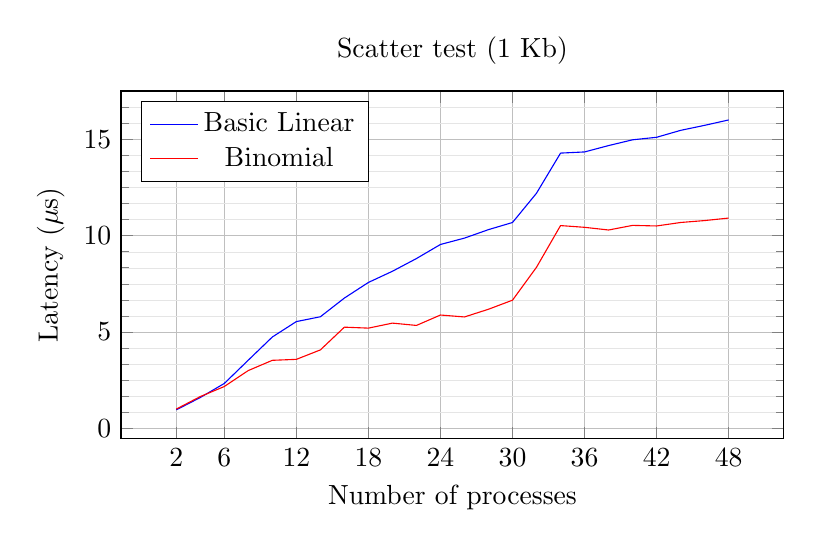
\begin{tikzpicture}
                \begin{axis}[
                    title={Scatter test (1 Kb)},
                    xlabel={Number of processes},
                    ylabel={Latency ($\mu$s)},
                    legend pos=north west,
                    grid=both,
                    grid style={line width=.1pt, draw=gray!20},
                    major grid style={line width=.2pt,draw=gray!50},
                    minor tick num=5,
                    xtick={2, 6, 12, 18, 24, 30, 36, 42, 48},
                    % xmode=log,
                    % log basis x={2},
                    % ymin=0,
                    % xmin=0.5,
                    % xmax=11.5,
                    % xmax=100,
                    % ytick={0, 50, 100, 150, 200, 250, 300, 350, 400},
                    width=10cm,
                    height=6cm,
                    % cycle list name=color list,
                ]
                
                % x = [ 2  4  6  8 10 12 14 16 18 20 22 24 26 28 30 32 34 36 38 40 42 44 46 48]
                % basic-linear = [ 0.96  1.6   2.33  3.54  4.74  5.54  5.79  6.76  7.57  8.15  8.81  9.54 9.87 10.31 10.68 12.2  14.28 14.34 14.67 14.97 15.1  15.46 15.72 16.  ]
                % binomial = [ 1.    1.65  2.17  3.    3.53  3.58  4.07  5.25  5.2   5.46  5.34  5.88  5.78  6.18  6.65  8.36 10.52 10.43 10.29 10.53 10.5  10.68 10.78 10.91]

                % Blue line: basic-linear
                \addplot[
                    color=blue,
                    mark=none,
                    ]
                    coordinates {
                    (2, 0.96)
                    (4, 1.6)
                    (6, 2.33)
                    (8, 3.54)
                    (10, 4.74)
                    (12, 5.54)
                    (14, 5.79)
                    (16, 6.76)
                    (18, 7.57)
                    (20, 8.15)
                    (22, 8.81)
                    (24, 9.54)
                    (26, 9.87)
                    (28, 10.31)
                    (30, 10.68)
                    (32, 12.2)
                    (34, 14.28)
                    (36, 14.34)
                    (38, 14.67)
                    (40, 14.97)
                    (42, 15.1)
                    (44, 15.46)
                    (46, 15.72)
                    (48, 16)
                    };
                    \addlegendentry{Basic Linear}

                % Red line: binomial
                \addplot[
                    color=red,
                    mark=none,
                    ]
                    coordinates {
                    (2, 1)
                    (4, 1.65)
                    (6, 2.17)
                    (8, 3)
                    (10, 3.53)
                    (12, 3.58)
                    (14, 4.07)
                    (16, 5.25)
                    (18, 5.2)
                    (20, 5.46)
                    (22, 5.34)
                    (24, 5.88)
                    (26, 5.78)
                    (28, 6.18)
                    (30, 6.65)
                    (32, 8.36)
                    (34, 10.52)
                    (36, 10.43)
                    (38, 10.29)
                    (40, 10.53)
                    (42, 10.5)
                    (44, 10.68)
                    (46, 10.78)
                    (48, 10.91)
                    };
                    \addlegendentry{Binomial}

                \end{axis}
            \end{tikzpicture}
            }
            % \resizebox{0.38\textwidth}{!}{
            % \begin{tikzpicture}
            %     \begin{axis}[
            %         title={Scatter test (1 Mb)},
            %         xlabel={Number of processes},
            %         ylabel={Latency ($\mu$s)},
            %         legend pos=north west,
            %         grid=both,
            %         grid style={line width=.1pt, draw=gray!20},
            %         major grid style={line width=.2pt,draw=gray!50},
            %         minor tick num=5,
            %         xtick={2, 6, 12, 18, 24, 30, 36, 42, 48},
            %         % xmode=log,
            %         % log basis x={2},
            %         % ymin=0,
            %         % xmin=0.5,
            %         % xmax=11.5,
            %         % xmax=100,
            %         % ytick={0, 50, 100, 150, 200, 250, 300, 350, 400},
            %         width=10cm,
            %         height=6cm,
            %         % cycle list name=color list,
            %     ]
                
            %     % x = [ 2  4  6  8 10 12 14 16 18 20 22 24 26 28 30 32 34 36 38 40 42 44 46 48]
            %     % basic-linear = [ 126.    222.22  357.39  479.9   623.76  789.07  902.46 1009.64 1117.33 1214.94 1334.99 1527.82 1572.21 1717.11 1846.12 2000.56 2118.62 2248.57 2355.12 2497.02 2571.44 2709.02 2796.63 2899.43]
            %     % binomial = [ 119.    383.83  655.32 1317.49 1628.77 2281.66 2964.79 3835.27 3795.96 4038.36 4238.62 5145.24 5513.75 5834.19 6527.81 7305.75 6995.97 7126.84 6804.27 7219.02 7201.17 7237.19 7771.69 8055.83]

            %     % Blue line: basic-linear
            %     \addplot[
            %         color=blue,
            %         mark=none,
            %         ]
            %         coordinates {
            %         (2, 126)
            %         (4, 222.22)
            %         (6, 357.39)
            %         (8, 479.9)
            %         (10, 623.76)
            %         (12, 789.07)
            %         (14, 902.46)
            %         (16, 1009.64)
            %         (18, 1117.33)
            %         (20, 1214.94)
            %         (22, 1334.99)
            %         (24, 1527.82)
            %         (26, 1572.21)
            %         (28, 1717.11)
            %         (30, 1846.12)
            %         (32, 2000.56)
            %         (34, 2118.62)
            %         (36, 2248.57)
            %         (38, 2355.12)
            %         (40, 2497.02)
            %         (42, 2571.44)
            %         (44, 2709.02)
            %         (46, 2796.63)
            %         (48, 2899.43)
            %         };
            %         \addlegendentry{Basic Linear}

            %     % Red line: binomial
            %     \addplot[
            %         color=red,
            %         mark=none,
            %         ]
            %         coordinates {
            %         (2, 119)
            %         (4, 383.83)
            %         (6, 655.32)
            %         (8, 1317.49)
            %         (10, 1628.77)
            %         (12, 2281.66)
            %         (14, 2964.79)
            %         (16, 3835.27)
            %         (18, 3795.96)
            %         (20, 4038.36)
            %         (22, 4238.62)
            %         (24, 5145.24)
            %         (26, 5513.75)
            %         (28, 5834.19)
            %         (30, 6527.81)
            %         (32, 7305.75)
            %         (34, 6995.97)
            %         (36, 7126.84)
            %         (38, 6804.27)
            %         (40, 7219.02)
            %         (42, 7201.17)
            %         (44, 7237.19)
            %         (46, 7771.69)
            %         (48, 8055.83)
            %         };
            %         \addlegendentry{Binomial}


            %     \end{axis}
            % \end{tikzpicture}
            % }
        \end{figure}

        \columnbreak

        For both message sizes, the binomial tree algorithm is faster
        than the basic linear algorithm. This was expected since it
        has a lower number of steps.
    \end{multicols}
\end{frame}



